\tcbsection{Resource Management and Development}

\subsection{D1 Resource Criterion}

The resources available to the school are sufficient to sustain the school program and are effectively used to carry out the school’s purpose and student achievement of the schoolwide learner outcomes, i.e., global competencies.

\subsubsection{Allocation Decisions}

\indicator{There is a relationship between the decisions about resource allocations, the school’s vision, mission and student achievement of the schoolwide learner outcomes and the academic histandards. The school leadership and staff are involved in the resource allocation decisions.}

\prompt{To what extent are resources allocated to meet the school’s vision, mission, and student achievement of the critical learner needs, the schoolwide learner outcomes and the academic standards? Additionally, comment on the extent to which leadership and staff are involved in the resource allocation decisions. What impact has the process for the allocation of resources made on student learning?}

\begin{findings}
Chiang Mai International School (\href{http://cmis.ac.th/}{CMIS}) continues to develop procedures and processes to ensure that the allocation of resources is in line with the \href{http://cmis.ac.th/about/vision}{school vision, mission statemen}t, student learning objectives (SLOs), curricular standards, and core values. 

The School Manager is responsible for the financial affairs of the school, human resources, purchasing, maintenance, gardening, and security with the help of the Assistant Manager. The Manager also oversees the functions of the office and management of the school budget along with the School Executive Team (SET). Through a standardized budgeting process, The School Executive Team (SET) prioritizes the most important education areas based on school-wide initiatives and divisional needs. The School Management Team (SMT), Teacher Leadership Team, and Directors are involved in the resource allocation decisions. 

CMIS Leadership has developed a \href{https://docs.google.com/document/d/1hh1nLUlJgg1hd7s6aG3u3We0L6o7Wg_ECdjc2f6DcT8/edit}{Curriculum Review process} in which specific evaluations tools, rubrics, and vetting instruments are used used to narrow down vendors and products for curricular and resource materials. CMIS Leadership also provides the necessary time and space required for teacher collaboration in vetting and evaluation of curricular items. CMIS Leadership will only allocate money for resources that are aligned to the standards, rigorous, and engaging and directly related to student achievement.  

The primary areas of \href{https://drive.google.com/a/cmis.ac.th/file/d/0B-CVlEN-TDChaEYxLWdWdHhqM3J6RzdGVlpFYmhIZnRvR3J3/view?usp=sharing}{budgetary allocation and expense} (in the General Fund) are Salary and Benefit (70\%), Instructional Expenses (7\%), Education Support (6\%), Utilities and Maintenance (5\%), Furniture and Equipment (2\%), and Student Welfare (1\%). 

CMIS is aligned with \href{https://drive.google.com/a/cmis.ac.th/file/d/0B-CVlEN-TDChaEYxLWdWdHhqM3J6RzdGVlpFYmhIZnRvR3J3/view?usp=sharing}{The Church of Christ in Thailand (CCT)} to establish the budget cycle, every October for the preliminary budget for the next school year and for the Final budget for the current school year.

Tuition and fees account for 99\% of annual income. For the past three years, tuition has increased at approximately 6-7\% annually for Standard and Discount Groups and 5\% for the Missionary Group. CMIS is a not-for-profit school; our tuition and fees are in the average range compared to other international schools in Chiang Mai for the Standard category and in the low range for the Missionary category.

The annual community survey, which is sent to parents, teachers, and students, is closely aligned with the school mission. This survey is given to all internal stakeholders (students, staff, and parents). The result of the survey showed that 42\% of ES teachers and 64 \% of MS and HS teachers have adequate IT support and resources.  In an effort to increase this area, the IT department has added Chromeboxes in the upper elementary classrooms and is sponsoring a Google Certified Educator Level 1 certification support for all staff. In addition, the IT working with the ES division to identify other ideas of how to further support them. At the time of the survey Middle School and High School students in grades 7, 8, and 9 received Chromebooks (as the second year of a three year implementation of 6-12). From the 2016-17 academic year forward, grades 6-12 receive school-provided Chromebooks. The 6-12 Chromebook program brings technology opportunities into all secondary classrooms and reduces the load on the elementary computer lab (previously used for middle school computer classes), allowing more access time to elementary students. Additionally, the IT department has moved to a ticketing system for support requests. These changes and additions should bring a positive impact to the need for IT support and resources.

{\centering
\includegraphics[width=\textwidth]{Chapter4_D1.jpg}}

\minor{So what...}

CMIS Leadership continues to involve multiple stakeholders in the resource allocation process. Steps have been taken to ensure resources are of high quality and are aligned to our standards. Though CMIS will continue to focus on resource allocation transparency, data indicates that more time and resources could be spent on improving the purchasing process and communication between teachers, leadership, and the purchasing department.  
\end{findings}

\subsubsection{Practices}

\indicator{The school develops an annual budget, has an annual audit, and at all times conducts quality business and accounting practices, including protections against mishandling of institutional funds.}

\prompt{Evaluate the school's processes for developing an annual budget, conducting an annual audit, and at all times conducting quality business and accounting practices, including protections against mishandling of institutional funds.}

\begin{findings}
CMIS has a clearly articulated, standardized budget process, ranging from August to July to comply with the Church of Christ in Thailand’s policy. 

\minor{Annual Budget}
 
The annual budget development is the responsibility of the School Manager and approved by the SET and the Board. During the budgeting process, the Manager seeks input from SMT, HODs, and Directors. The Preliminary Budget for the next school year has to be approved by the SET and sent to the Board for approval and then to the Foundation of the Church of Christ in Thailand (CCT) for approval in October. The Final Budget of the current school year has to be approved by the SET, then sent to the Board, and finally to the CCT in the same month.

Within this budget process, the Board has a long-term projection on enrollment that determines the staffing of full-time equivalent (FTE) and part-time teacher and staff. The revised organization structure for the next school year is presented to the Board in February - March. For foreign staff, the Superintendent normally sends a letter of intent in December and asks them to reply by January the next year which allows foreign hire employment contracts to be issued by late January in order to finalize the school’s recruiting needs. The job posting will be started from February until the positions are filled.

Once the budget is approved by the CCT, the SET is responsible for its implementation and the Manager monitors day-to-day budget expenditures and other financial matters. Monthly Financial Reports are sent to the Board for approval. The Board is not involved in the day-to-day financial or operational affairs of the school.

The Finance Advisory Committee is approved by the Board every three years. The committee meets and makes a recommendation to the Board to approve tuition and fees for the three-year scheme. After the Board approves, the Tuition scheme will be announced to parents. The Finance Advisory Committee is comprised of the SET, one parent representative from Missionary group, one parent representative from a non-Missionary group, Head of Finance Department, and one Board member.

The School Executive Team search data from member schools of East Asia Regional Council of Schools (\href{https://www.earcos.org/}{EARCOS}), International School Association of Thailand (\href{https://www.isat.or.th/index.php}{ISAT}), and Chiang Mai Circle of International Schools (CMCIS, ISCN) for salary and benefits data from benchmark schools to determine that CMIS’s salary and benefits (S\&B) are fair and equitable. 

For salary and benefits, the SET discusses and finalizes the next two-year plan with Teacher and Administrative  Communication Team (\href{https://docs.google.com/document/d/14nhwcw8xo3i-23Q-WUxo6KJ_c8yFKu-jTdCctt4MFcs/edit}{TACT}) for foreign staff and with the Head of Departments for Thai staff. Then the SET recommends it to the Board to approve before sending an announcement to all staff in December.

\minor{External and Internal Audits}

Annually, CMIS conducts external audits by an external firm approved by the CCT in October and by the CCT Internal Auditor in November. After both groups approve the audit, the SET will recommend to approve the allocation of Net Income Over Expenses to the Board. Net Income Over Expenses is then reinvested into the CMIS Specific Funds (i.e. retirement, human resources, and emergency)and Plant Fund (i.e. building, furniture, and technology). The external and internal audits also prevent unintentional misuse of CMIS funds. 

\minor{Quality Business and Accounting Practices}

The Board performs the following duties to safeguard the financial stability of CMIS:
\begin{itemize}
\item approves monthly and annual financial reports 
\item approves clear policies recommended by the SET and changes in any policies
\item approves school-wide investment
\item monitors processes and procedures for business operations to comply with the CCT policy.
\end{itemize}

\minor{So what...}

CMIS has several internal and external structures in place to ensure the development of an annual budget, an annual audit, and at all times conducts quality business and accounting practices, including protections against mishandling of institutional funds.

CMIS Leadership should continue to maintain and monitor CMIS auditing, budgetary, and accounting practices. 
\end{findings}

\subsubsection{Facilities}

\indicator{The school’s facilities are adequate, safe, functional, and well-maintained and support the school’s mission, desired learner goals, and educational program.}

\prompt{Evaluate the adequacy of the facilities in relation to the health and safety needs of students and supporting the school’s mission, desired learner goals and educational program.}

\begin{findings}
CMIS facilities are safe, functional, and well maintained. 

\minor{Current Location and \href{http://blogs.cmis.ac.th/campus/}{New Development Plan}}

The CMIS Board of Directors approved to stay on current CMIS campus in March 2014 and it was announced to the CMIS community by the Board Chairman. The community survey was conducted in April 2015 and included the topic of a Campus Development Plan to seek input and priorities from the community. The \href{http://blogs.cmis.ac.th/campus/}{CMIS Campus Development Plan} was approved by the Board in July 2015 and shared with community at the beginning of 2015-16 school year. The plan covered both the renovation of existing facilities and the construction of new buildings and facilities which is estimated to finish during the 2018-2019 school year.

Facility and furniture planning is factored into the long-term financial planning and budgeting process. To ensure the facilities and furniture remain adequate, money is set aside in the Capital Fund to support future needs.

\minor{Safety, Functionality and Security}

\begin{itemize}
\item CMIS considers safety and security as top priorities for its students and employees. We contain and/or maintain the following:
\item Yearly emergency plan; \href{https://docs.google.com/document/d/1bWb3k7yCv7oRx52dS9tLZe_e0DhaAsxz8f1OxJD2-is/edit}{periodic fire and lockdown drills}; fire alarms testing; fire extinguisher system; new school-wide PA system; a new CCTV system at Specific Point (IT Office and Guard Box); contracted G4S guard service.
\item Playgrounds that are multi-age appropriate that encourage interaction between all students and promote the school mission of creating a caring and welcoming environment.
\item Safety report for playground equipment
\item Several annual maintenance contracts with professional contractors for air-conditioning, and CCTV network.
\item In 2016 CMIS constructed a security fence around the school, changed a guard box and added more CCTVs, with a \href{http://blogs.cmis.ac.th/newsletter/2016/05/13/service-of-thanksgiving-for-the-security-wall-grant-given-by-the-united-states-of-america/}{grant from the US government}.
\item The facilities for instructional programs include classroom space for each teacher, a library, a gym and playing field. 
\end{itemize}

\minor{Site Adequacy }

In general, CMIS’s current facilities are adequate to meet current student involvement in both curricular and co-curricular programs. CMIS enrollment is close to capacity and as student numbers grow, there will be an increasing demand to find additional classrooms, more space in the library, additional laboratories, a larger PE field, and play area. The CMIS campus development plan for the next three years will address these needs.

In the last three years, significant funding has been allocated to develop, upgrade, and maintain the quality of the buildings, infrastructure, and furniture. The master plan for campus development and renovation is periodically reviewed and shared to community to best support education program and the continued growth of the school at all levels.

\minor{So What...}

Though the CMIS site is currently adequate for the current student population, the campus would benefit from a larger playing fields, additional covered play spaces, as well as an aquatics facility. Additionally, data suggests that CMIS Leadership could study the feasibility of improving the learning environment of some of the high school classrooms by improving wall space and furniture. 
\end{findings}

\subsubsection{Instructional Materials and Equipment}

\indicator{The policies and procedures for acquiring and maintaining adequate instructional materials and equipment, such as textbooks, other printed materials, audio-visual, support technology, manipulatives, and laboratory materials are effective.}

\prompt{Evaluate the effectiveness of the policies procedures for acquiring and maintaining adequate instructional materials and equipment, such as technology tools and software, the support systems for technology, software, textbooks, other printed materials, manipulatives, and laboratory materials for instruction including online.}

\begin{findings}
CMIS Leadership maintains and monitors policies and procedures for acquiring and adequate instructional materials. 

\minor{\href{https://docs.google.com/document/d/1hh1nLUlJgg1hd7s6aG3u3We0L6o7Wg_ECdjc2f6DcT8/edit}{Curriculum Review Cycle}}

Since curricular decisions should be made using clear standards and student outcomes as a guide, a new Curriculum Review Cycle/Resource Adoption strategic plan had to be developed and implemented. The most important elements of the Curriculum Review process are the specific evaluations tools, rubrics, and vetting instruments that have been developed and used to narrow down vendors and products for curricular and resource materials. CMIS Leadership also provides the necessary time and space required for teacher collaboration in vetting and evaluation of curricular items. 

Science curriculum was the first content to be vetted and evaluated based upon the \href{https://docs.google.com/document/d/1hh1nLUlJgg1hd7s6aG3u3We0L6o7Wg_ECdjc2f6DcT8/edit}{Curriculum Review Cycle}; science curriculum was purchased during the 2015-2016 school year. As with ELA curriculum decisions, science saw significant conceptual changes with the adoption of the the Next Generation Science Standards. Because of this, CMIS Leadership, developed vetting and evaluation instruments to ensure curriculum and resource alignment with the standards, as well as rigor and student engagement. This year, Mathematics undertook the same curriculum vetting process and ELA/social studies will be reviewed next year. 

In order to ensure that the resources we purchase outside of the normal adoption cycle are of the highest quality and they meet our three general criteria of: is it aligned to the standards? Is it rigorous? and is it engaging? \href{https://docs.google.com/a/cmis.ac.th/forms/d/e/1FAIpQLSfyvc6GwQkO6mVo-x6Lani_ezs_ZnHfgG_EgiPXXJbmkxt19g/viewform?c=0&w=1}{Resource Request} and \href{https://docs.google.com/a/cmis.ac.th/forms/d/e/1FAIpQLSd7lRTi5wYEb9tdis-jbgqyoo3poS_TdJCWU_2BQkKJknAvFA/viewform?c=0&w=1}{Resource Renewal forms} were developed and implemented. 

To acquire new resources outside of the normal adoption cycle, teachers submit a Resource Request form. The information submitted on the form is used by the Curriculum Director, Superintendent, and the School Manager to determine quality: alignment to standards, rigor, and engagement. 

For non-instructional materials and resources, teachers fill out a \href{https://docs.google.com/document/d/1X2HU8VcgV48m1ZY_-3AztVdD8j5VwBu6O319_9W825M/edit}{School Supply Form}  (for supplies on site) or the  \href{https://docs.google.com/document/d/125eFGQt3dRQkHOhyhMHIx6Eup4jG9Zc4B2mYjvgxpqg/edit}{Supply Requisition Form} (for supplies purchase outside of CMIS) The information on the form is used by the Principal and School Manager to evaluate. If approved, the form is given to the Purchasing Supervisor to begin the purchasing process.

All delivered resources (i.e. textbooks, \href{https://docs.google.com/spreadsheets/d/1T_vMmATtxHEartDVy76fRwgws8cWChwxHOLEDzgGyEc/edit?ts=589d58a6#gid=0}{IT inventories}, musical instruments), the Purchasing Officer will label them before distributing them to teachers. Textbooks and IT inventory (i.e. Chromebooks) are also catalogued online using the \href{http://library.cmis.ac.th/}{Koha system}. 

\minor{Resource and Technology Budget}
 
The budgets for instructional materials and technology purchases are developed annually in order to support the school’s purpose and student achievement. CMIS allocates 7\% of its annual budget to the instructional expenses. Through the annual budgeting process, the SET seeks input from \href{https://docs.google.com/document/d/1iW_tWIwRlWU2p0oIOvd3usDsxj9qYDt_2ROwNPBTHSc/edit}{Teacher Leadership Team} members, Principals, and Curriculum Director to establish an estimated budget for textbooks, instructional materials, and resources.

CMIS has gone through a great deal of improvement in technology since the last self study. For example, CMIS Leadership has addressed some technology needs through the 1:1 Chromebook initiative. All students in grades 6 through 12 have been assigned Chromebooks for the academic year. All classrooms have an LCD projector and wireless access. All teachers have laptops since 2014-15 school year giving them the mobility in the classroom and allowing them to participate in professional development effectively,  assisting in the delivery of instruction, and managing data. The budget for technology is a part of the overall resource budget and plans are in place to satisfy future technology needs.

\minor{So what...}

CMIS has several policies and procedures in place for acquiring and maintaining adequate instructional materials and equipment.

Though processes and policies are in place to address resource and material adoption, there has been a lack of understanding of certain budgetary, ordering, and approval process by teachers and staff. This has caused some confusion and delay in resource allocation. CMIS Leadership is in the process of clarifying, simplifying, and communicating these procedures.
\end{findings}

\subsubsection{Well-Qualified Staff}

\indicator{Resources are available to enable the hiring, nurturing, and ongoing professional development of a well-qualified staff for all programs such as online instruction and college/career.}

\prompt{Determine if the resources available enable the hiring, nurturing, and ongoing professional development of a well-qualified staff for all programs, such as online instruction and college/career.}

\begin{findings}
CMIS believes that teachers and staff are our most important resources. We also understand that maintaining faculty and staff is a year-round process. Consequently, CMIS utilizes a number of resources for hiring and nurturing a well-qualified staff. More specifically, CMIS has increased resources for hiring as well as improved the professional development program (Faculty Handbook pp 46-47) and the \href{https://docs.google.com/document/d/1dN2nFzb_NHUekvrnmY0A3ttMZoVuJKn4iRhvfT4j6go/edit}{new staff orientation program}. A consistent and rigorous interviewing process is applied during recruitment via both Skype and in-person interviews if possible.  

CMIS has made it a priority to ensure that new hired teachers are appropriately qualified and certified in their home countries. CMIS Leadership is currently ensuring that those teacher certifications and qualifications are maintained and in good standing. Furthermore, CMIS Leadership has also ensured that all new hired teachers go through a criminal background check and/or fingerprint clearing from their home countries. 
 
CMIS offers \href{https://docs.google.com/a/cmis.ac.th/forms/d/1zUFhXdeDp45qEERn_zrdiv0whW8qaKVmAy51M27IGu4/edit}{letters of early intent} which results in the school having advanced notice of vacancies for the upcoming school year. This allows administrators to start the recruitment process in February. 

\minor{Attracting and Retaining Qualified Staff}

To attract and retain qualified staff, CMIS realizes that compensation, benefits, and professional development funds are important and ensure that 70\% of the operating budget allocated for Salary and Benefit. With that in mind, the SET has researched information from many sources (i.e. international schools in Chiang Mai and Bangkok and EARCOS salary survey) to verify that our salary and benefit package are comparable and competitive. 

The Board approved and announced the salary increase for foreign staff (i.e.certified /licensed counselors and certified /licensed teachers) by one and a half steps for two school years (2016-2017, 2017-2018). One new benefit also was approved: an Attendance Incentive (i.e. CMIS pays for personal days that are not used - maximum 5 days). Teacher Leadership Team members stipend per semester was also increased 33\% from 7,500 baht to  10,000 baht per semester. Other benefits that will be maintained at an appropriate and acceptable level are: the housing allowance, outpatient and inpatient insurances, and tuition benefit for staff children.

\minor{Professional Development}

CMIS reserves around 43,000 USD for Professional Development Fund annually. This fund is used for schoolwide needs. Staff can choose the professional development they are interested to join and send to the Superintendent to approve. The school also provides in-house professional development during our Wednesday Early Release Day monthly. See sections on Collaborative Work, Research Based Knowledge, Professional Collaboration, and Professional Development for more information on CMIS professional development findings. High-quality professional development opportunities are identified and disseminated to the faculty both in-house and from outsource trainings. 

\minor{Nurturing Staff}

During the last school year, CMIS has established the New Staff Committee. The main objective of this committee is to create a smooth transition for all new staff and help them prepare all necessary paperwork to get their visas and work permits. CMIS Leadership as also created the New Hire Buddy Program make the personal transition to Chiang Mai as seamless as possible. New staff begin the school year earlier than returning staff to participate in \href{https://docs.google.com/document/d/1dN2nFzb_NHUekvrnmY0A3ttMZoVuJKn4iRhvfT4j6go/edit}{New Staff Orientation} programs and Thai Culture training curriculum.  The SET and the Director of Curriculum plan for new and returning teacher orientations. The Sunshine Committee also helps in promoting congenial work relationship by acknowledging birthdays and other significant events in the CMIS Staff community.  

CMIS Leadership is currently analyzing teacher workloads to ensure an acceptable balance between teaching and preparation time. \href{https://docs.google.com/document/d/18CUFZg0GClP-o7cAknyvsH9G6yivTofi1E_OwdvHHt4/edit}{Exit Interviews and Surveys} are also used for future improvements.
 
\minor{So what...}

CMIS has worked hard to ensure that appropriate resources are available to enable the hiring, nurturing, and ongoing professional development of a well-qualified staff. CMIS Leadership understands the need to continuously evaluate and prioritize foreign teacher  compensation and benefits to encourage them to extend their stay in CMIS. Professional development opportunities are a priority at CMIS and will be emphasized in the future planning process. Finally, CMIS Leadership will continue to hire only teachers that are appropriately certified, qualified, and have been thoroughly vetted for child safety positions. 
\end{findings}

\subsubsection{Conclusions}
\prompt{Comment on the degree to which this criterion is being addressed.}

CMIS addresses this criterion to a high degree. The processes of training, hiring, nurturing, and vetting highly qualified teaching candidates will be monitored and maintained, as will the current resource management and adoption procedures. CMIS Leadership will continue to work to develop processes with stakeholders on teacher workload balance and compensation. 

\minor{Maintain and Monitor}

\begin{itemize}
\item Processes and instruments used in resource evaluation and curriculum review. 
\item Annual budget processes
\item Internal and external audit processes 
\item Safety and security protocols
\item Process in place to hire, nurture, and vet high qualified staff. 
\end{itemize}

\minor{Continue to Improve}
\begin{itemize}
\item Purchase and ordering processes
\item Building and facilities-including site adequacy
\item Professional development opportunities that are aligned differentiated to deliberate practice 
\end{itemize}


\subsection{D2 Resource Planning Criterion}

The governing authority and the school leadership execute responsible resource planning for the future.

\subsubsection{Long-Range Resource Plan}

\indicator{The school has developed and implemented a long-range resource plan. The school has a process for regular examination of this plan to ensure the continual availability of appropriate resources that support the school’s vision, mission, and student learning of schoolwide learner outcomes and academic standards.}

\prompt{Evaluate the process for regular examination of the long-range resource plan to ensure the continual availability of appropriate resources that support the school's vision, mission, and student learning.}

\begin{findings}
CMIS Leadership has developed and implemented a long-range resource plan that ensures high quality resources that are aligned to the standards, rigorous, and engaging. 

\minor{Long Term Financial Plan}

CMIS has a Long-Term Financial Plan (LTFP) that includes predicted educational resources and facility needs. Sufficient funds are allocated to ensure that critical resources are maintained in the future, including emergency and capital improvement funds. School-wide and divisional educational initiatives are funded through annual budgets, which are part of the LTFP.

CMIS’s LTFP also includes a three-year forward cash flow statement showing projected revenues and expenses based off the aligned assumptions (e.g., enrollment and major capital projects).The capital improvement fund is intended to support future facility development that includes completing the new high school building, library and cafeteria building, a swimming pool and upgrading facilities. CMIS’s LTFP includes a long-term IT master resource plan that includes budgeting and replacement cycles. The CMIS Manager and Assistant Manager develop an annual facility maintenance, renovation, and modification plan. As part of the budget building process, the Board reviews the key facility and maintenance projects and costs.

The Board meets annually to consider long-term strategic objectives and needs of the school. To ensure responsible planning for the future, the Board has worked to address the long-term, outstanding matters related to school goals, Vision and Mission, and school Identity and Core Values.

\minor{Long Term Resource Adoption Cycle }

The CMIS Resource Adoption Cycle provides all stakeholders information and a timeline on which departments in what school year should focus on adoption. This Resource Cycle allows CMIS Leadership to be transparent to staff and community and have a written, strategic plan to address changes in standards/research, assess our needs as related to mission/vision, and make informed decisions about curriculum and resources. 

During the adoption year, all CMIS Teaching Staff that are responsible for teaching that particular content will be involved in the adoption processes, if possible. In general, the process involves teacher groups completing a need analysis, unpacking of the standards, depth of knowledge analysis (to address rigor), and resource evaluation using content specific evaluation tools and rubrics (to address standard alignment). The evaluation tools must be research based and aligned with the standards in mind. 

Though the \href{https://docs.google.com/document/d/1hh1nLUlJgg1hd7s6aG3u3We0L6o7Wg_ECdjc2f6DcT8/edit}{CMIS Resource Adoption Cycle} clearly outlines which academic year each department should expect a formal resource analysis, some departments, such as music, art, and physical education, have yearly budgets due to the consumable nature of their resources and materials. 

CMIS has used the Adoption Process for two years. Last year science teachers K-12 engaged in the process and this year, all math teachers completed it. 

In order to ensure that the resources we purchase outside of the normal adoption cycle are of the highest quality and they meet our three general criteria of: is it aligned to the standards? Is it rigorous? and is it engaging? Resource Request and Resource Renewal forms were developed and implemented. See sections Current Educational Research and Thinking and Curricular Review, Revision, and Evaluation sections for more information. 

\minor{So what...}

CMIS Leadership will continue to maintain and monitor all long term plans, including curriculum/resource adoption and finances. Currently, Schoolwide Learner Outcomes, Mission/Vision, and academic standards are in good standing and will be similarly monitored and maintained. 
\end{findings}

\subsubsection{Use of Research and Information}

\indicator{The school uses research and information to form the master resource plan.}

\prompt{To what extent does the school leadership and staff use research and information to form the long-range plan?}

\begin{findings}
CMIS Leadership utilizes data from multiple sources to inform the Master Resource Plan

CMIS’s annual community, \href{https://docs.google.com/forms/d/e/1FAIpQLSdPiMWntLfKwp7ZHpiOoIshADmvSlH50TI0Mi_RVzvtcOnDoQ/viewform?c=0&w=1}{IT}, and \href{https://drive.google.com/drive/u/0/folders/0B7w2qeag9D8cT0J0YlFlUDdnMXc}{after-event surveys} are critical sources of information. Results of the survey on many topics such as  resources and activities are reviewed and lead to subsequent improvement. All surveys have been developed annually.

CMIS uses annual benchmark data for salaries and benefits, tuition, and enrollment to help form the assumptions for the annual budget and for the LTFP. External sources such as exchange rate, economic data, and inflation rate are also taken into considerations.

\minor{So what...}

CMIS currently uses research and community feedback to make informed decision about the master resource plan.
Currently, plans can be found in different locations and formats. This makes it difficult to evaluate and assess for effectiveness. CMIS plans to create a central location in a format that is consistent and easy to access.
\end{findings}

\subsubsection{Involvement of Stakeholders}

\indicator{Stakeholders are involved in the future planning.}

\prompt{Evaluate the effectiveness of the involvement of stakeholders in the school's future planning.}

\begin{findings}
CMIS Leadership and Staff ensure that there is effective involvement of all stakeholders in the school’s future planning. CMIS Leadership identifies stakeholders as: students, teachers, parents, support staff, administrators, the Board and the surrounding community. 

The following are examples of how internal and external stakeholders are involved with CMIS future planning: 

\begin{itemize}
\item The Board develops annual goals and these goals are shared out with the community by the School Executive Team (SET).
\item SET meets every week and School Management Team (SMT) meets every other week to review upcoming events and assign individual responsibilities to share out with the community.
\item Beginning in 2015, CMIS utilized Students, Staff and Parents Focus Groups to brainstorm ideas and gain insights. 
\item \href{https://www.facebook.com/cmis.th/photos/pcb.536310393230874/536309946564252/?type=3&theater}{PTG (Parent Teacher Group)} regularly meet with staff, administrators, and community members. At the beginning of the 2016-17 school year, the PTG sent out a \href{https://docs.google.com/document/d/1kiwakkg8eKdtEexCxVNx-m1CfC3VqxhukDy8WXDPGKY/edit?ts=58a2a142}{parent survey} asking them to identify future topics for PTG meetings.
\item Teacher Leadership Team Members meet monthly with administrators to review future goals and plans for level of support.
\item Student Communication Groups are held  bi-monthly and at times students are asked to share perceptions of school wide processes and policies. 
\item Superintendent meets with Student Council (Stuco) representative every semester to discuss upcoming plans.
\item \href{http://blogs.cmis.ac.th/ptg/2016/12/05/agenda-ptg-general-meeting-december-6th-2016/}{Parent Coffee Mornings} in which parents meet with administrators and staff to discuss future schoolwide plans. 
\item CMIS Teaching Staff regularly communicate with parents regarding students progress and future educational plans. 
\item \href{http://blogs.cmis.ac.th/newsletter/2016/09/05/super-thursdays-starts-this-week/}{Super Thursday} meetings in which the Superintendent meets informally with parents to discuss school improvement.  
\item Regular staff meeting structures: department, divisional,  and ad hoc committees. 
\item \href{https://drive.google.com/drive/folders/0B0TYmzaZNi3fRW56VWtIOGFLUFU?usp=sharing}{Parent-Teacher Conferences} are organized once a semester to plan student achievement. 
\end{itemize}

CMIS  conducts an annual community survey which all CMIS parents, students, and staff are asked to participate. The survey collects both quantitative and qualitative data. All internal stakeholders have a voice through this survey. The Community Survey ask for quantitative data on family demographics and marketing. Perceptual data about the Board, administrators, and teachers is also collected.  

\minor{So what...}

CMIS Leadership and Staff provide multiple opportunities for all internal and external stakeholders to participate in the CMIS community. CMIS Leadership and Staff would benefit from greater time and resources to analyze the survey data, especially the Community Survey. A CMIS Data Sandbox would be especially helpful in making survey data accessible and user friendly. 
\end{findings}

\subsubsection{Informing}

\indicator{The governing authorities and school leaders are involved in informing the public and appropriate governmental authorities about the financial needs of the organization.}

\prompt{Comment on the evidence that the governing authority and school leaders are involved in informing the public and appropriate governmental authorities about the financial needs of the organization.}

\begin{findings}
CMIS Leadership inform the public and appropriate governmental organizations as necessary. Though informing the public or governmental organization of financial needs is not required, CMIS Leadership does ensure important financial information is communicated to certain community members.  
For example, The Board’s letter to parents announcing the new comprehensive tuition and fee structure explained the relationship between these costs and the level of educational services provided.

CMIS reports monthly to CCT, in which financial state and future plans impacting the finances are made known.

Several times each year, the SET meets with the full faculty to inform them about the major school developments and school finances. The School also posts \href{http://blogs.cmis.ac.th/newsletter/}{newsletters} to inform the parents and community about key \href{https://docs.google.com/document/d/1ksBWJ56c42PXtYU3laOebWdo_Jz3J56XZAKVm8s_Lpg/edit}{school developments}.

\minor{So what...}

As a private school, CMIS is not required to inform governmental authorities about the financial needs of the organization. CMIS leadership understands the need for communication and regularly updates the community of school investment and development.
\end{findings}

{\centering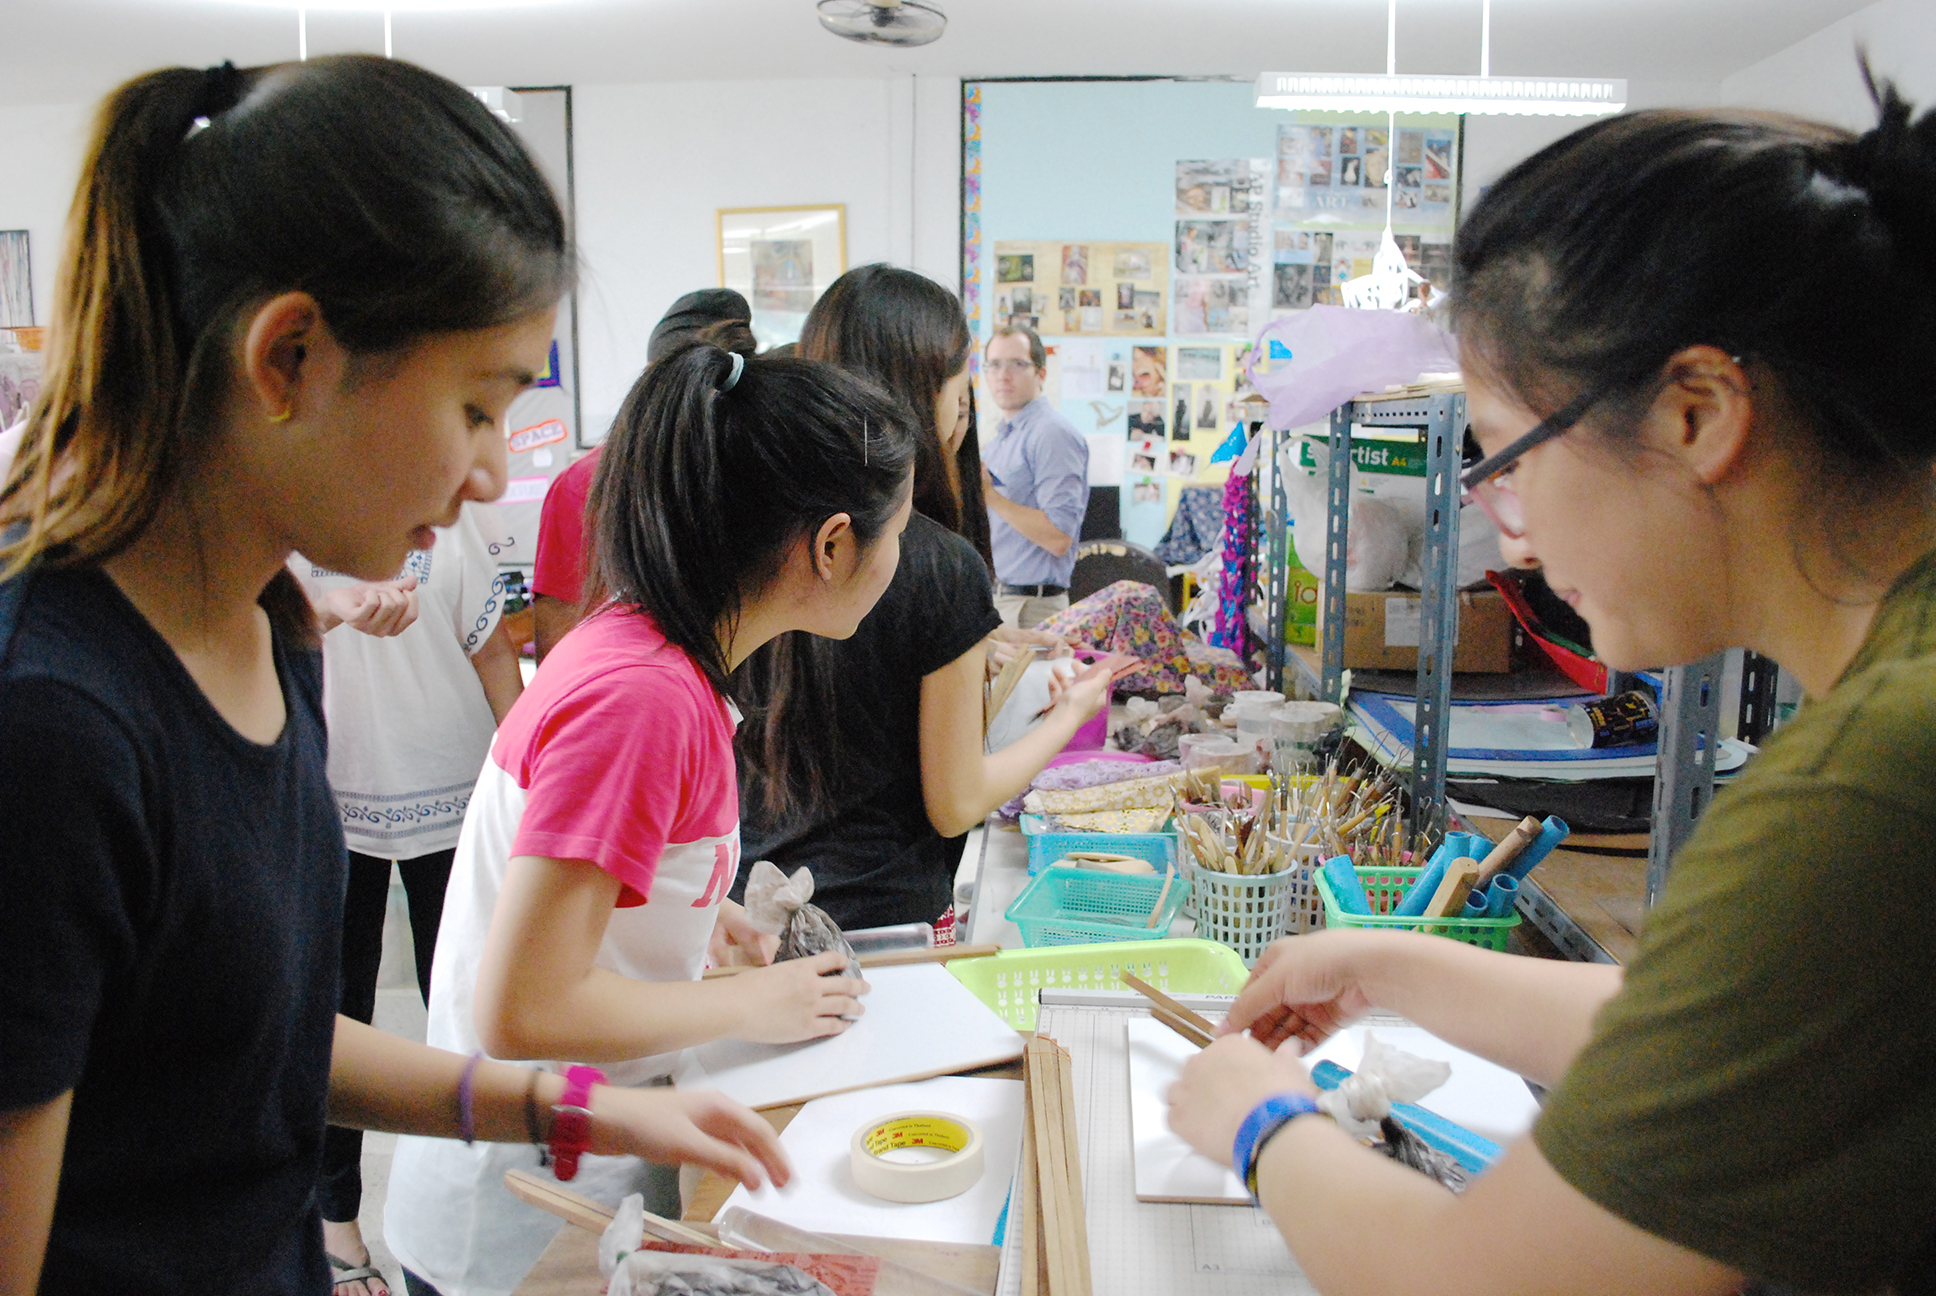
\includegraphics[width=\textwidth]{Chapter4_D2.jpg}}

\subsubsection{Marketing Strategies}

\indicator{The school has marketing strategies to support the implementation of the developmental program.}

\prompt{How effective are the marketing strategies to support the implementation of the developmental program?}

\begin{findings}
CMIS has a well-known reputation in Northern Thailand among missionaries, government personnel, the broader
expatriate community, and educated Thais.

To maintain this reputation, the school carries out several public relations and marketing initiatives. The school manager has been responsible for public relations, marketing, and community outreach since 2013-2014. Subsequently, the PR Committee was formed. The PR team leader is the Manager and team members include the Admission Director, IT officer, and PR assistant. From 2015-2016, the Student Support staff was invited to join the committee as well. 

The committee’s goal is to create PR activities, branding plans, and a budget based on the School Vision, Mission, Schoolwide Learner Outcomes, and the Board’s goals. The committee meets every other week during the school year to exchange ideas and follow up with plans and budgets.

Main activities of the committee:

\begin{itemize}
\item The \href{http://cmis.ac.th/}{school website}’s new user interface from 2016-2017
\item Launching and maintaining school Facebook sites (\href{https://www.facebook.com/cmis.th/}{CMIS general}, \href{https://www.facebook.com/cmis.eagles}{CMIS Eagles}, \href{https://www.facebook.com/cmis.alumni/}{CMIS Alumni})
\item Advertising and \href{http://www.chiangmaicitylife.com/citylife-articles/wow-what-a-year/}{news flashes} in City Life for Chiang Mai community outreach, \href{https://drive.google.com/a/cmis.ac.th/file/d/0B-CVlEN-TDChRkhmUTBnNjhaLUtvUDNCcm16eEdmYkFKWFk0/view?usp=sharing}{Expat life magazine} for the Bangkok community outreach, and \href{https://drive.google.com/a/cmis.ac.th/file/d/0B-CVlEN-TDChNWJ2NFZwM0QyR0U/view?usp=sharing}{TIE both online and newspaper}
\item Creating \href{https://www.youtube.com/channel/UCqVO5ckeUjOrxI1ElQaXM3g}{videos} of school history, \href{http://blogs.cmis.ac.th/newsletter/}{important events}, activities, and student and alumni interviews to put on the website
\item Booths to promote school (e.g. The International Conference of Mission, The Church of Christ in Thailand Mission day,  \href{https://www.facebook.com/cmis.th/photos/a.184627431732507.1073741831.175187506009833/465899696938611/?type=3&theater}{International Balloon Festival}, \href{http://blogs.cmis.ac.th/newsletter/2016/08/17/cmis-participating-thailand-international-mathematics-school-model-exhibition-2016/}{International Math Competition})
\item \href{https://docs.google.com/a/cmis.ac.th/forms/d/1basukpCBjcCMWXDh-cUUWW6lgk6zxYadGMn1EzFDQwc/edit}{New family survey} in September (started SY 2015-16)
\item \href{https://drive.google.com/drive/folders/0B0TYmzaZNi3fU3JWR2FFbndiR2s?usp=sharing}{Open House for prospective families} in early Elementary school (e.g. Teddy Bear Picnic, Garden party, Jungle party)
\end{itemize}

Apart from the activities of the PR committee, the Manager, Admissions Director and Superintendent recently attended an ISAT sponsored marketing conference together: \href{http://www.isat.or.th/news/isat-professional-development-workshop}{Boosting Enrollment in a Competitive Market}. They are currently working on strategies for sharing out their learning from this training and highlighting ways to for CMIS constituent groups to support and advance CMIS future development.

\minor{Educational Organizations}

To maintain educational excellence, strengthen our network, and promote the school, CMIS has been a member of a number national and international educational organizations, including :

\begin{itemize}
\item The International Schools Circle of North (ISCN)
\item The International School Association of Thailand (\href{http://gallery.cmis.ac.th/2016-2017/ISAT-Regional-Meeting/}{ISAT})(the School Manager is a committee member)
\item The East Asia Regional Council of Schools (\href{https://www.earcos.org/}{EARCOS})
\item The International Educator (\href{https://www.tieonline.com/}{TIE})
\item \href{https://www.collegeboard.org/}{The College Board}
\item Association of Christian Schools International (\href{https://www.acsi.org/}{ACSI})
\item The Association for Supervision and Curriculum Development (\href{http://www.ascd.org/Default.aspx}{ASCD})
\item Academy for International School Heads (\href{http://www.academyish.org/}{AISH})
\item National Association of Independent School (\href{http://www.nais.org/Pages/default.aspx}{NAIS}) 
\end{itemize}

\minor{Networking Regionally}

CMIS Superintendent and Curriculum Director have been invited every year to be \href{http://www.earcos.org/etc2017/etc-teachers.php}{presenters at EARCOS conference}s since 2014-2015. Their trainings have focussed on research based data analysis processes, teacher observation tools, and classroom instructional strategies. 

The Curriculum Director has organized multiple \href{http://blogs.cmis.ac.th/newsletter/2016/11/29/cmis-sponsors-earcos-mathematics-workshop/}{workshops for EARCOS} and at other international schools in Bangkok and in Chiang Rai. CMIS also received a grant from EARCOS to organize a Math workshop in Chiang Mai. There were 10 International Schools from Thailand and other countries to join this workshop.

\minor{Student-centered Public Relations}

CMIS provides a number academic, students centered programs that not only benefit the student intellectually, but are also opportunities for CMIS to network with other international schools. Since 2014, CMIS has been involved with \href{http://blogs.cmis.ac.th/newsletter/2016/03/21/cmis-student-take-top-awards-in-the-south-asia-division-of-the-national-history-day-competition/}{National History Day}, each year CMIS send a teacher representative to Jakarta to help with the regional competition and share CMIS students’ projects. \href{http://gallery.cmis.ac.th/2016-2017/MUN/}{Model United Nations} is another academic program that promotes CMIS in Chiang Mai and Chiang Rai. Finally, the many \href{http://blogs.cmis.ac.th/community-service/}{Community Service} activities the students are \href{http://blogs.cmis.ac.th/newsletter/2016/11/10/cmis-community-service-at-northern-school-for-the-blind/}{involved} in is another positive avenue for networking and marketing the school. 

For the outreach to \href{https://www.facebook.com/cmis.alumni/}{Alumni} community and \href{http://cmis.ac.th/support}{donors}, the school hired a new part-time Alumni coordinator and a Development Consultant starting from SY 2016-17. We hope that these two positions will create more activities to promote the school and increase more donations for Campus Development Plan as well as other important developments of the school.

\minor{So what...}

CMIS should continue to maintain and monitor the marketing programs that are in good standing. It should also continue to keep abreast with current trends for international schools (e.g., 64\% of international schools are in Asia, the number of international schools in Chiang Mai has tripled over last 10 years) and use this data as a basis for future marketing strategies. 
\end{findings}

\subsubsection{Conclusions}
\prompt{Comment on the degree to which this criterion is being addressed.}
CMIS Leadership addresses this criterion to a high degree. Stakeholders play a key role in the school’s future planning and the school has involved all stakeholders in the planning for the improvement of student learning. Resources are planned and provided according to the allocated budget, which may be adjusted when needed.

\minor{Maintain and Monitor }

\begin{itemize}
\item Long term financial planning processes
\item Adopted curriculum that is aligned to adopted standards. 
\item Adoption review cycle, resource request form, resource renewal form.
\item Course offering that ensure rigor, relevance, and coherence. 
\item Structures to ensure alignment of standards to actual concepts through vetted curriculum, adjustments to UbDs, instructional rounds, formal evaluations, and blueprints. 
\item Assessment alignment to standards and rigor of standards. 
\item Programs, curriculum, and planning that requires authentic integrations among disciplines (NHD, PARCC, UdD) 
\item Emphasis of looking at student work as data to make curricular and instructional decisions.\end{itemize}

\minor{Continue to improve}

\begin{itemize}
\item Aligning resource management and development to Schoolwide Learner Outcomes as appropriate 
\item Increased communication with all stakeholders
\item Research based marketing and public relation strategies
\item Identifying additional ways to evaluate effectiveness of resource management and development
\end{itemize}
